\documentclass[11pt,a4paper]{article}
\usepackage[utf8]{inputenc}
\usepackage[french]{babel}
\usepackage[T1]{fontenc}

\usepackage{amsmath}
\usepackage{amsfonts}
\usepackage{amssymb}

\newcommand{\TitreMatiere}{Algorithmique et Structures de Données 1}
\newcommand{\TitreSeance}{Pointeurs}
\newcommand{\NumeroTD}{Structures \& Pointeurs}
\newcommand{\DateCours}{Octobre 2022}
\newcommand{\AnneeScolaire}{2022-2023}
\newcommand{\Organisation}{EPITA}
\newcommand{\NomAuteurA}{Fabrice BOISSIER}
\newcommand{\MailAuteurA}{fabrice.boissier@epita.fr}
\newcommand{\NomAuteurB}{ }
\newcommand{\MailAuteurB}{ }
\newcommand{\DocKeywords}{Algorithmique}
\newcommand{\DocLangue}{fr} % "en", "fr", ...

\usepackage{MetalQuickLabs}

% Babel ne traduit pas toujours bien les tableaux et autres
\renewcommand*\frenchfigurename{%
    {\scshape Figure}%
}
\renewcommand*\frenchtablename{%
    {\scshape Tableau}%
}

% Ne pas afficher le numéro de la légende sur tableaux et figures
\captionsetup{format=sanslabel}


\begin{document}

\EncadreTitre

\bigskip


%\begin{center}
%\begin{tabular}{p{5cm} p{11cm}}
%\textbf{Commandes étudiées :} & \texttt{sh}, \texttt{bash}, \texttt{man}, \texttt{ls}, \texttt{mkdir}, \texttt{touch}, \texttt{chmod}, \texttt{mv}, \texttt{rm}, \texttt{rmdir}, \texttt{cat}, \texttt{file}, \texttt{which}, \texttt{which}\\
%
%\textbf{Builtins étudiées :} & \texttt{pwd}, \texttt{cd}, \texttt{exit}, \texttt{logout}, \texttt{echo}, \texttt{umask}, \texttt{type}, \texttt{>}, \texttt{>{}>}, \texttt{<}, \texttt{<{}<}, \texttt{|}\\
%
%\textbf{Notions étudiées :} & Shell, Manuels, Fichiers, Répertoires, Droits, Redirections\\
%\end{tabular}
%\end{center}

\bigskip


Ce document a pour objectif de vous familiariser avec les pointeurs, c'est-à-dire avec la mémoire et les adresses en mémoire.

%\bigskip
\medskip

Définition informelle d'un pointeur~\footnote{Wikipedia : \href{https://fr.wikipedia.org/wiki/Pointeur_(programmation)}{Pointeur}} : \og \textit{En programmation informatique, un pointeur est un objet qui contient l'adresse mémoire d'une donnée ou d'une fonction} \fg .

\medskip

Dans les différents exercices précédemment faits, vous avez régulièrement utilisés les tableaux et des index pour sélectionner une case à l'intérieur pour accéder au contenu.
Les pointeurs fonctionnent exactement comme les index : il s'agit de l'adresse d'une case dans un tableau externe à toutes les fonctions et variables manipulées jusqu'à présent.

%\medskip
\smallskip

Les pointeurs travaillent en \textit{mémoire}, c'est-à-dire dans un espace de stockage indépendant des variables et du contexte des fonctions.
Lorsqu'une fonction est appelée, les paramètres sont copiés vers le contexte de la fonction et l'espace dédié aux variables est créé.
Lorsqu'une fonction est terminée (par un \textit{return}) ou une procédure (on termine l'exécution de la dernière instruction de la procédure), l'espace réservé pour les variables et les paramètres est libéré.
Ainsi, les variables et paramètres ne peuvent exister que lors de l'exécution de la fonction/procédure qui les exécute.

Dans l'exemple suivant, les variables et paramètres n'existent que dans leur contexte.
Seul le paramètre \textit{y} fait en réalité référence à la variable \textit{j} de la fonction \textit{FonctionA} (\textit{y} renvoie vers \textit{j}).


\begin{table}[h!]
  \centering
  \begin{minipage}{0.45\textwidth}
    \centering
% %*   *)
\begin{lstlisting}[style=algorithmique]
FonctionC : entier
  parametres locaux
    entier  z
  variables
    entier  m, n
m = 1
n = 2
retourner(m + n + z) // 3 + z

ProcedureB : entier
  parametres globaux
    entier  y
  variables
    entier  a,b
a = FonctionC(0)     // a = 3
b = 2
y = a + b            // j = y = 5

FonctionA : entier
  parametres locaux
    entier  x
  variables
    entier  i, j
FonctionB(j)         // (j = 5)
i = j + x            // i = 5 + x
retourner(i)         // 5 + x \end{lstlisting}
    % \caption{Algorithme de la somme des N premiers entiers}
    % \label{algo-somme-n-premiers-entiers}
  \end{minipage}
  \hfillx
  \begin{minipage}{0.5\textwidth}
    \centering
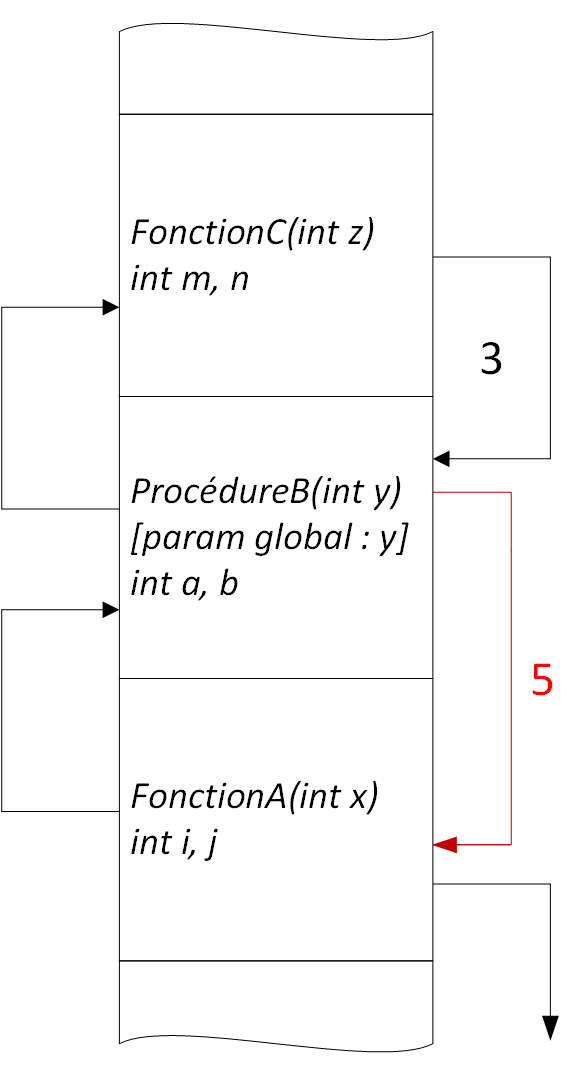
\includegraphics[width=0.75\textwidth]{img/pointeurs/pile_appels_seule.png}
  \end{minipage}
%  \caption{Algorithme de la somme des N premiers entiers}
%  \label{somme-n-premiers-entiers}
\end{table}


\pagebreak


Dans les ordinateurs, la \textit{mémoire} est l'espace où peuvent être stockées des données lors de l'exécution des programmes.
On sépare généralement la \textit{mémoire} (l'espace où l'on stocke les données dont l'accès doit être immédiat) de la \textit{mémoire de masse} (l'espace où l'on stocke les données dont l'accès peut être différé et/ou dont le volume est trop gros pour entrer en mémoire vive).

Pour illustrer, dans une bibliothèque, il est nécessaire d'avoir accès instantanément à la liste des livres appartenant à la bibliothèque, lesquels sont disponibles en rayon, et dans quel rayon les trouver, ou éventuellement lesquels sont disponibles en réserve.
Dans ce cas, l'index doit être en \textit{mémoire vive}, et les livres en \textit{mémoire de masse} : on cherche d'abord si le livre est disponible et où il se trouve, avant de chercher parmi tous les rayons et les livres existants.

Toujours dans l'exemple de la bibliothèque, le livre serait la donnée visée, et sa côte (le numéro de référence indiquant le rayon où le trouver) serait sont adresse, donc un pointeur faisant référence à ce livre.

\bigskip

La mémoire est donc l'espace où l'on stocke les données, et un pointeur est littéralement une adresse (ou référence) vers une case de cet espace.
Dans l'exemple suivant, on a donc la mémoire représentée comme un grand tableau, et ici, on a un pointeur avec l'adresse $ 44 $ qui fait référence à une case contenant la valeur $ 91 $.

\bigskip

\begin{center}
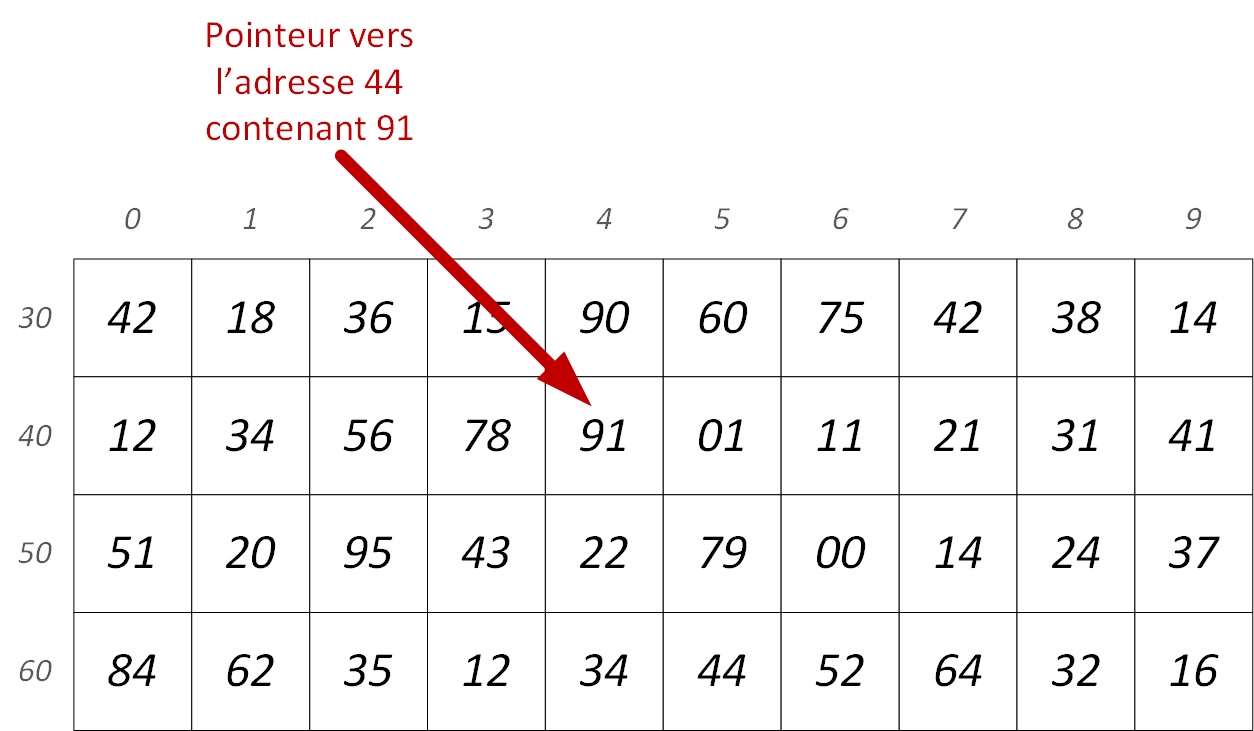
\includegraphics[scale=0.75]{img/pointeurs/memoire_pointeur.png}
\end{center}

\bigskip

Pour déclarer une variable comme étant un pointeur, on utilise l'opérateur $ * $ après le nom du type.
Par exemple pour un pointeur vers un entier, on va déclarer :

\bigskip

\begin{table}[h!]
  \centering
  \begin{minipage}{0.45\textwidth}
    \centering
% %*   *)
\begin{lstlisting}[style=algorithmique]
variables
  int   i
  int   *ptr
\end{lstlisting}
    % \caption{Algorithme de la somme des N premiers entiers}
    % \label{algo-somme-n-premiers-entiers}
  \end{minipage}
  \hfillx
  \begin{minipage}{0.5\textwidth}
    \centering
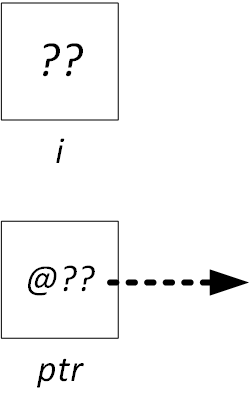
\includegraphics[scale=0.75]{img/pointeurs/pointeurs0_1_type.png}
  \end{minipage}
%  \caption{Algorithme de la somme des N premiers entiers}
%  \label{somme-n-premiers-entiers}
\end{table}

\bigskip

Les déclarations se lisent de la droite vers la gauche.
On peut donc lire ces deux variables comme étant : \textit{i est un entier, ptr est un pointeur vers un entier}.

\medskip

Pour \textit{déréférencer} un pointeur, c'est-à-dire pour accéder à la valeur dans la case visée, on utilise également l'opérateur $ * $, mais d'une autre manière.

\bigskip

\begin{table}[h!]
  \centering
  \begin{minipage}{0.45\textwidth}
    \centering
% %*   *)
\begin{lstlisting}[style=algorithmique]
variables
  int   i
  int   *ptr

ptr = malloc(sizeof (int))
(*ptr) = 42
i = (*ptr) \end{lstlisting}
    % \caption{Algorithme de la somme des N premiers entiers}
    % \label{algo-somme-n-premiers-entiers}
  \end{minipage}
  \hfillx
  \begin{minipage}{0.5\textwidth}
    \centering
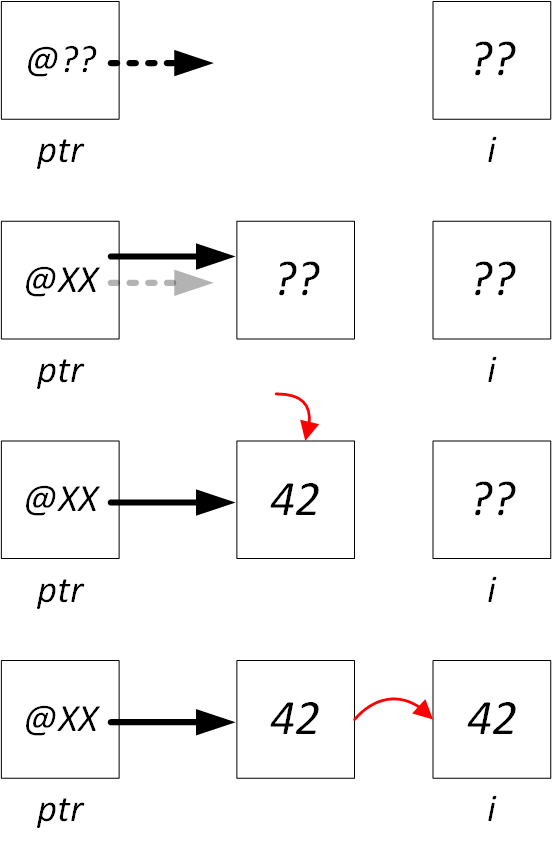
\includegraphics[scale=0.75]{img/pointeurs/pointeurs0_2_dereferencements.png}
  \end{minipage}
%  \caption{Algorithme de la somme des N premiers entiers}
%  \label{somme-n-premiers-entiers}
\end{table}

\bigskip

Ici, on demande au système de nous donner une case mémoire pouvant accueillir un entier.
Le système se débrouille pour trouver un espace de taille suffisante, puis, il renvoie l'adresse de cette case (\textit{ptr} récupère donc l'adresse de cette case).

Ensuite, on indique que l'on déréférence la variable \textit{ptr} pour y mettre $ 42 $.
C'est-à-dire que l'on indique que l'on résout l'adresse de \textit{ptr} pour accéder à la case visée, puis, on y met la valeur $ 42 $.

La dernière ligne indique que l'on déréférence \textit{ptr} (on résout l'adresse de \textit{ptr}) pour récupérer la valeur au bout et la mettre dans la variable \textit{i}.
Maintenant, \textit{i} contient donc $ 42 $.

\bigskip

On peut également \textit{faire référence à} une variable ou autre.
Pour cela, on va utiliser l'opérateur $ \& $.

\begin{table}[h!]
  \centering
  \begin{minipage}{0.45\textwidth}
    \centering
% %*   *)
\begin{lstlisting}[style=algorithmique]
variables
  int   i
  int   *ptr

ptr = &i
i = 42
(*ptr) = 8 \end{lstlisting}
    % \caption{Algorithme de la somme des N premiers entiers}
    % \label{algo-somme-n-premiers-entiers}
  \end{minipage}
  \hfillx
  \begin{minipage}{0.5\textwidth}
    \centering
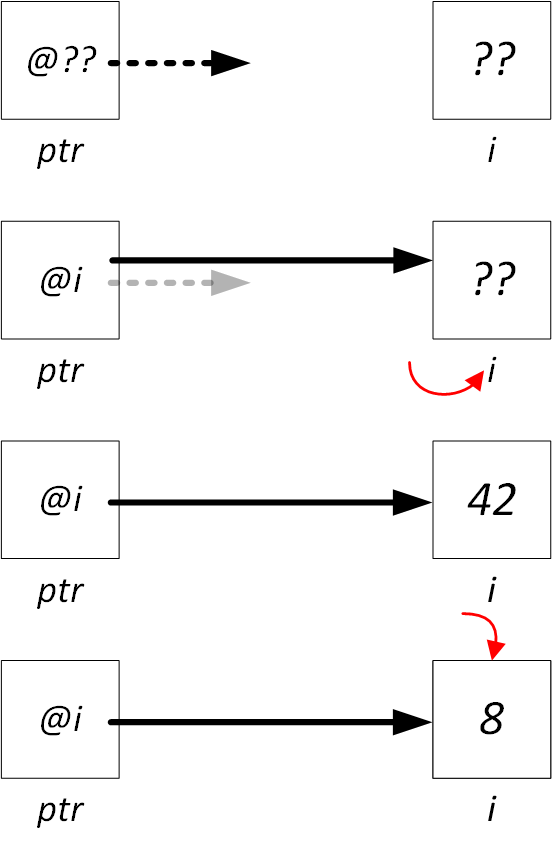
\includegraphics[scale=0.75]{img/pointeurs/pointeurs0_3_references.png}
  \end{minipage}
%  \caption{Algorithme de la somme des N premiers entiers}
%  \label{somme-n-premiers-entiers}
\end{table}

Ici, on indique que \textit{ptr} va prendre l'adresse permettant de pointer vers \textit{i}.
\textit{ptr} a donc pris une référence vers \textit{i}.
On remarque que \textit{ptr} n'a pas été déréférencé : c'est normal, \textit{ptr} est une adresse, et on lui donne l'adresse vers \textit{i}.

Ensuite, dans la deuxième ligne, on met la valeur $ 42 $ dans \textit{i}.
Si on déréférence \textit{ptr}, on y trouvera donc $ 42 $.

La dernière ligne indique que l'on va mettre $ 8 $ dans la case pointée par \textit{ptr}.
Comme \textit{ptr} pointe vers la variable \textit{i}, on est train de mettre $ 8 $ dans \textit{i}.
Finalement, \textit{i} contient donc $ 8 $.


\pagebreak
\vfillFirst


Pour résumer avec un schéma distrayant, on peut tout simplement repenser au concept d'adresse dans le monde réel.

\begin{center}
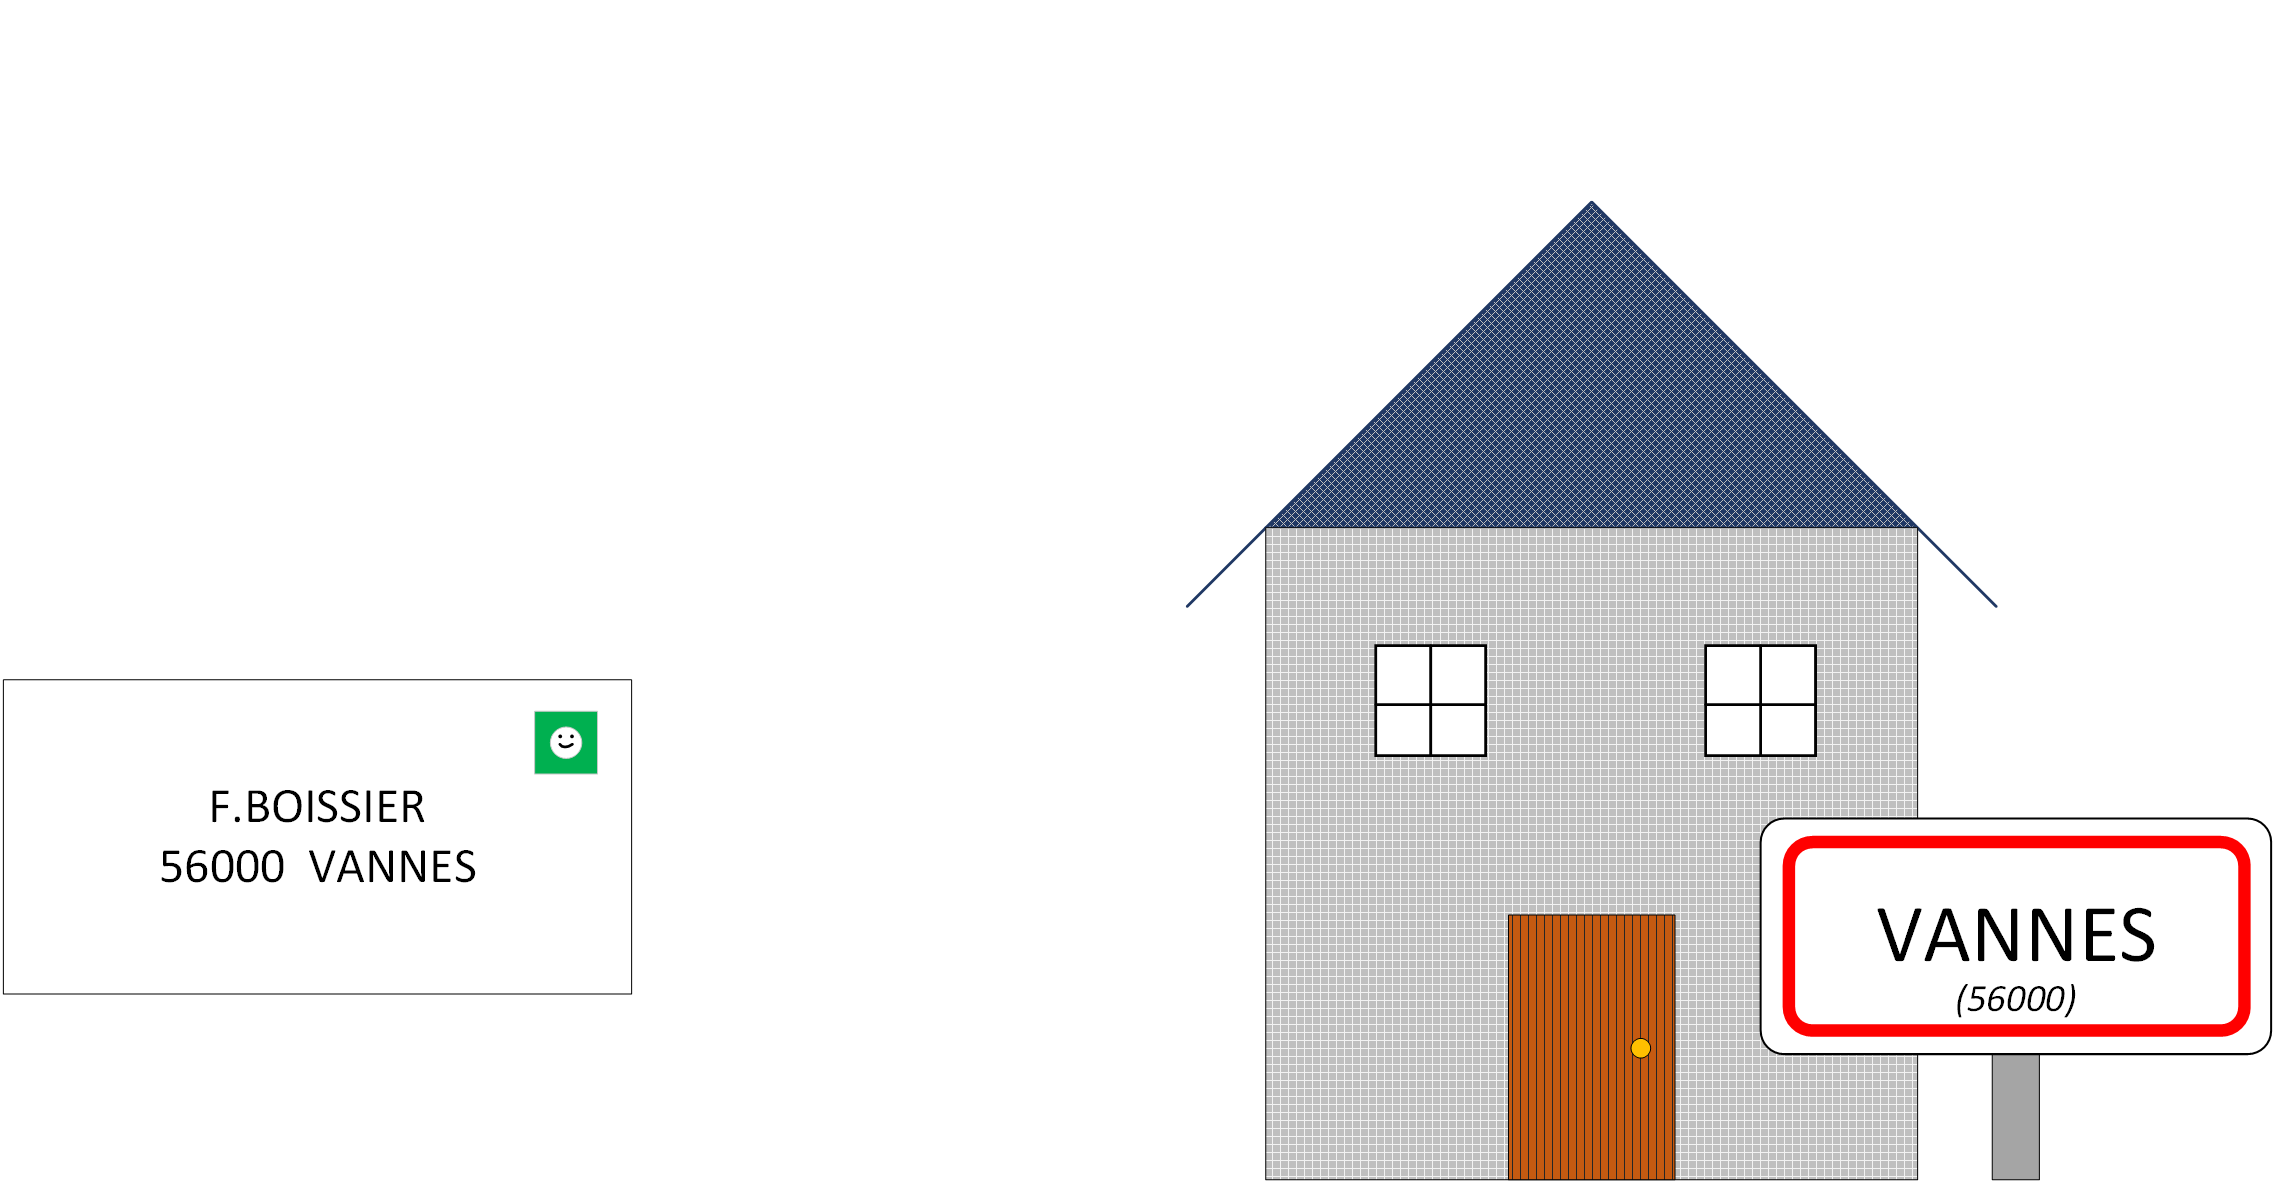
\includegraphics[width=\textwidth]{img/pointeurs/pointeurs_ville.png}
\end{center}

\begin{itemize}
\item L'adresse sur l'enveloppe est un pointeur vers une maison très précise. \\

\item Chaque maison (ou case mémoire) est physiquement à une seule adresse précise. \\

\item Lorsque la Poste prend l'enveloppe et lit l'adresse pour pouvoir livrer le courrier au bon endroit, elle est en train de \textit{déréférencer} l'adresse vers la maison qui doit recevoir l'enveloppe.
La Poste est donc en train d'effectuer une opération similaire à ce que ferait cette expression : \underline{$ (*\text{adresse}) $} ou en mettant la vraie valeur : \underline{$ (*56000) $} \\
(Vous vous rendez également compte que le code postal $ 56000 $ correspond en réalité à Vannes) \\

\item À l'inverse, lorsque quelqu'un vous demande où vous habitez, cette personne vous demande une \textit{référence vers} votre maison, c'est-à-dire votre adresse.
En donnant l'adresse de votre logement, vous êtes en train de donner une référence vers votre maison comme le ferait l'expression : \underline{$ \&(\text{Ma Maison}) $} c'est-à-dire l'adresse et le code postal \underline{$ 56000 $} \\
(Donner la référence vers ma maison, c'est donner l'adresse de mon logement, donc indiquer que j'habite à Vannes avec le code postal $ 56000 $) \\

\item Si vous indiquez à la Poste de rediriger vers une autre adresse tous les courriers arrivant à votre adresse, alors vous vous rapprochez du concept où l'on définit des pointeurs de pointeurs : \underline{$ **\text{adresse} $} \\
(Le premier déréférencement accède bien à une case, mais celle-ci contient une adresse indiquant en fait qu'il faut déréférencer de nouveau pour atteindre la maison/l'emplacement réel de la donnée) \\
\end{itemize}


\vfillLast
\pagebreak

Dans peu de temps, vous allez implémenter les listes chaînées à base de pointeurs.
Cette structure de données permet de prendre des éléments et les stocker à des positions précises, puis de les sortir de la liste selon leur position ou d'autres critères.
Fonctionnellement parlant, il s'agit donc de stocker des éléments dans un certain ordre, comme dans le schéma suivant :

\begin{center}
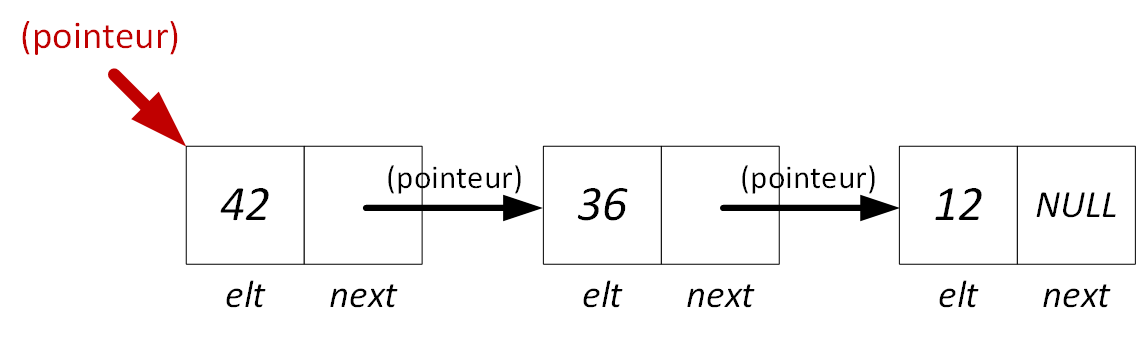
\includegraphics[scale=0.75]{img/pointeurs/pointeurs1.png}
\end{center}

Vous pouvez observer que la structure de données contient à la fois un élément et un pointeur vers le maillon suivant.
Le dernier maillon dispose d'un pointeur \textit{NULL}.

Cette valeur \textit{NULL} est spéciale, car lorsqu'on la déréférence, cela déclenche une erreur.
Il ne faut donc JAMAIS la déréférencer.
Par contre, c'est une valeur remarquable que l'on peut tester.

Ainsi, avant de déréférencer un pointeur, ou lorsque l'on veut constater que l'on est au dernier élément de la liste, on teste si le pointeur est à \textit{NULL} ou pas.

\medskip

Revenons sur la mémoire, les pointeurs, et la liste chaînée.
Pour stocker en mémoire cette liste, il a fallu appeler la fonction \textit{allouer} (ou \textit{malloc} en C) pour chaque maillon ajouté.
Cette fonction demande au système de trouver de l'espace et de le donner au programme.
Vous ne pouvez quasiment pas deviner où se trouve cette case en mémoire.
Si votre programme a fait énormément d'allocations en mémoire et de libérations de la mémoire, alors les éléments peuvent se trouver à des endroits très distincts/des espaces non contiguës.

L'image suivante illustre cela : le maillon contenant l'élément $ 42 $ est à l'adresse $ 30 $, le maillon suivant contenant l'élément $ 36 $ se trouve à l'adresse $ 32 $, et enfin, le dernier maillon contenant l'élément $ 12 $ se trouve à l'adresse 63 (on notera que c'est le dernier élément parce que le pointeur vers l'élément suivant a l'adresse \textit{NULL}).

\begin{center}
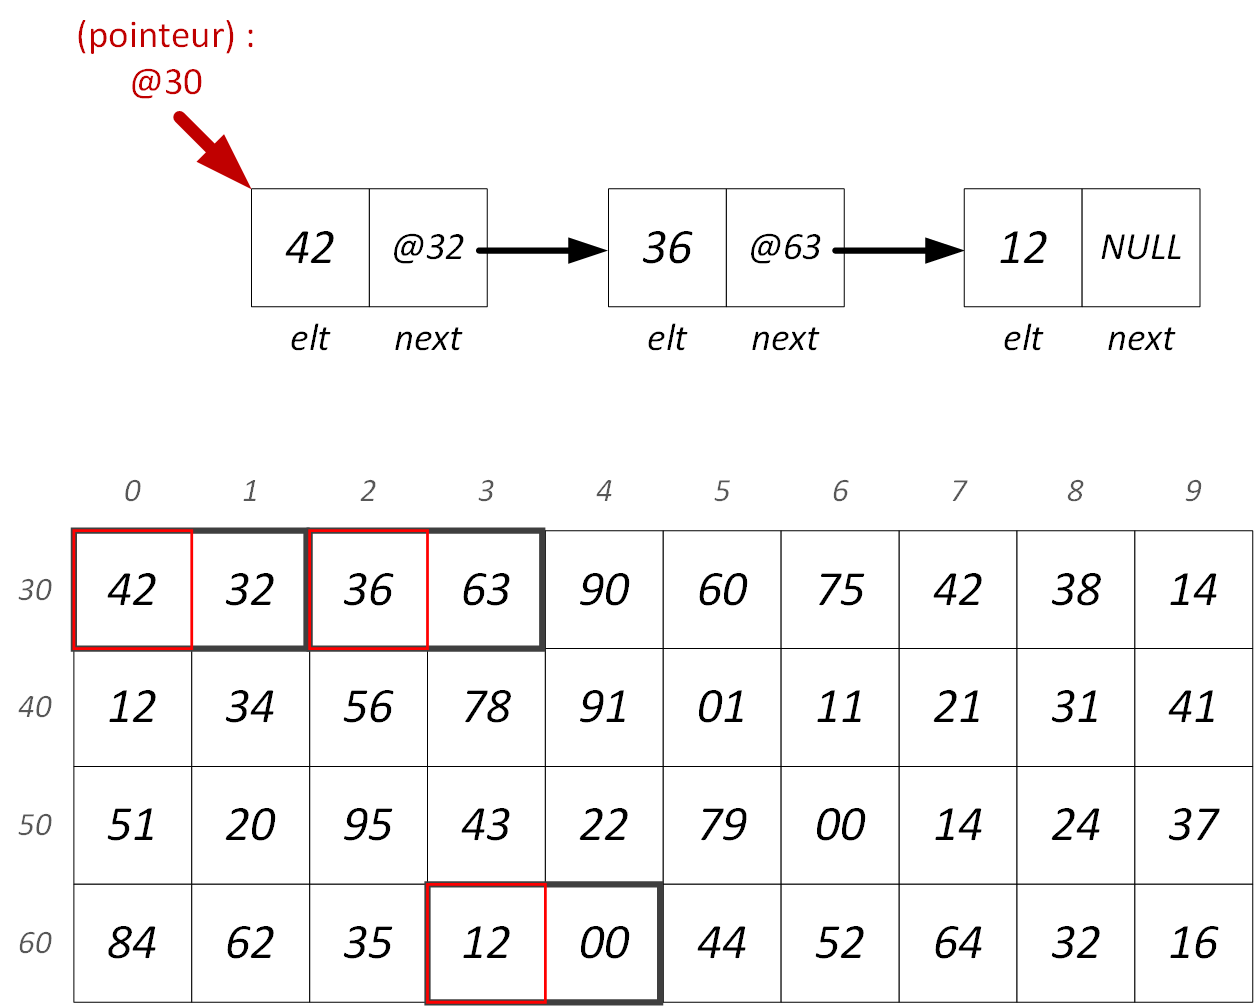
\includegraphics[scale=0.85]{img/pointeurs/pointeurs2.png}
\end{center}

Ainsi, les pointeurs sont simplement des \textit{adresses} vers des cases mémoire ($ int *ptr $), et lorsque l'on souhaite accéder à la donnée au bout de l'adresse/au bout du pointeur on effectue un \textit{déréférencement} ($ (*ptr) $).

Pour retrouver l'adresse d'un élément que l'on manipule, on demande une \textit{référence vers} cet élément ($ ptr = \&i $).


\bigskip

\vfillFirst

\vfillLast


\begin{center}
\textit{Ce document et ses illustrations ont été réalisés par Fabrice BOISSIER en octobre 2022}
\end{center}

\end{document}
